\documentclass{ctexrep}
\usepackage[margin=25mm]{geometry}
\usepackage{amsmath}
\usepackage{fancyhdr}
\usepackage{cite}
\usepackage{graphicx}
\usepackage{float}
\usepackage{indentfirst}
\usepackage[utf8]{inputenc}
\usepackage{amssymb}
\usepackage{hyperref}
\hypersetup{
colorlinks=true,
linkcolor=black
}

\usepackage{titlepic}
\providecommand{\keywords}[1]
{
  \small	
  \textbf{\textit{关键词}} #1
}










%\usepackage[linesnumbered,boxed]{algorithm2e}
\usepackage{listings}
\usepackage{xcolor}

\definecolor{codegreen}{rgb}{0,0.6,0}
\definecolor{codegray}{rgb}{0.5,0.5,0.5}
\definecolor{codepurple}{rgb}{0.58,0,0.82}
\definecolor{backcolour}{rgb}{0.95,0.95,0.92}

\lstdefinestyle{mystyle}{
    backgroundcolor=\color{backcolour},   
    commentstyle=\color{codegreen},
    keywordstyle=\color{magenta},
    numberstyle=\tiny\color{codegray},
    stringstyle=\color{codepurple},
    basicstyle=\ttfamily\footnotesize,
    breakatwhitespace=false,         
    breaklines=true,                 
    captionpos=b,                    
    keepspaces=true,                 
    numbers=left,                    
    numbersep=5pt,                  
    showspaces=false,                
    showstringspaces=false,
    showtabs=false,                  
    tabsize=2
}

\lstset{style=mystyle}


\pagestyle{fancy}
\chead{贪吃蛇}


\begin{titlepage}
    \titlepic{
\includegraphics[width=0.4\textwidth]{9.jpg}}
    
    \title{2021年春季学期
    
数据结构课程设计A3题实验报告
}
%A^{b}

\author{
张津赫*\footnotemark[1], 曹伟\footnotemark[1], %对应同一个脚注符号
张天浩\footnotemark[1], %\Envelope
}
    %\author{
%张津赫^{1*}%,%曹伟^{1}%, %张天浩^{1}% 软件学院2019级8班
%}
    \date{软件学院2019级8班
}

    
    
    
\end{titlepage}


\begin{document}
\definecolor{mygreen}{rgb}{0,0.6,0}
\definecolor{mygray}{rgb}{0.5,0.5,0.5}
\definecolor{mymauve}{rgb}{0.58,0,0.82}
\lstset{ %
backgroundcolor=\color{white},   % choose the background color
basicstyle=\footnotesize\ttfamily,        % size of fonts used for the code
columns=fullflexible,
breaklines=true,                 % automatic line breaking only at whitespace
captionpos=b,                    % sets the caption-position to bottom
tabsize=4,
commentstyle=\color{mygreen},    % comment style
escapeinside={\%*}{*)},          % if you want to add LaTeX within your code
keywordstyle=\color{blue},       % keyword style
stringstyle=\color{mymauve}\ttfamily,     % string literal style
frame=single,
rulesepcolor=\color{red!20!green!20!blue!20},
% identifierstyle=\color{red},
language=c++,
}














\maketitle















\begingroup
    \fontsize{14pt}{16pt}\selectfont
      
       
    
\begin{abstract}
\hspace{1cm}利用极大极小树与alpha-beta剪枝算法结合,限定层数为6层,并采用$c++$ $STL$ 类的list类型,对蛇体信息进行存储,该算法对比贪心方法,简单评估函数有很大提升。

\vspace{1cm}\hspace{0.3cm}
\textbf{\emph{关键词}}(alpha-beta剪枝,缓存增强试探法,散列表)



\end{abstract}

\endgroup



\maketitle  % 生成 Summary Sheet
\tableofcontents  % 生成目录


\chapter{分工与合作
}
1.张津赫:参与实现alpha-beta剪枝函数,细节修改,mtdf实现,bug调试。
\vspace{0.5cm}

2.张天浩: 主要负责alpha-beta剪枝函数实现,bug调试。
\vspace{0.5cm}

3.曹伟:   参与实现alpha-beta剪枝函数,负责评估函数的实现 ,bug调试。

\vspace{1cm}


\begin{itemize}

\item 4.17 讨论简单的贪心算法,算法局限性较大,难以提高效率。

\item 4.18 转而简单评估函数,胜率较低。

\item 4.20 选择alpha-beta剪枝+缓存增强试探法+散列表,进行研讨,开始着手进行代码编写。

\item 成功完成代码,并成功运行。




\end{itemize}

\chapter{算法思想}
\section{总体思路}
 本题程序主要使用了Alpha-Beta剪枝算法, Alpha-Beta剪枝算法是对Minimax方法的优化,它们产生的结果是完全相同的,只不过运行效率不一样。Alpha-Beta只能用递归实现。这个思想是在搜索中传递两个值,第一个值是Alpha,即搜索到的最好值,任何比它更小的值就没用了,因为策略就是知道Alpha的值,任何小于或等于Alpha的值都不会有所提高。

如果某个着法的结果大于Alpha但小于Beta,那么这个着法就是走棋一方可以考虑走的,除非以后有所变化。因此Alpha会不断增加以反映新的情况。有时候可能一个合理着法也不超过Alpha,这在实战中是经常发生的,此时这种局面是不予考虑的,因此为了避免这样的局面,我们必须在博弈树的上一个层局面选择另外一个着法。

这个算法严重依赖于着法的寻找顺序。如果你总是先去搜索最坏的着法,那么Beta截断就不会发生,因此该算法就如同最小-最大一样,效率非常低。该算法最终会找遍整个博弈树,就像最小-最大算法一样。
在AlphaBeta剪枝算法中,因为存在剪枝,搜索过程并不完整,所以剪枝算法所得到的估值不一定是准确值。由此可看出,alpha-beta剪枝算法重点关注的是(alpha,beta)区间,它也称为搜索窗口。相对于alpha节点和beta节点而言,程序搜索PV节点的过程是比较费时的。如果把搜索窗口的宽度减小,发生剪枝的可能性就会加大,程序搜索的时间也会短些。在选择每一次的试探值时,通常的想法是采用二分法,即每次都选择估值区间的中点进行试探。采用二分法的效率确实比较高,但是荷兰计算机科学家Aske Plaat经研究发现,在多次搜索试探过程中,局面估值往往会出现在前一次搜索的返回值附近,而机械地选取中点做为新的试探值并不是最高效的。于是他提出了一种选取前一次搜索返回值做为新试探值的MTD算法(Memory-enhanced Test Driver,缓存增强试探法)——MTD(f)。

增加可搜索的节点数量。蛇的位置采用c++ STL类的list类型进行实时更新。该算法从网站得到基本的结构,随后根据网站内呈现的基本结构逐步扩充代码,完成了蛇的移动与溯源,估值函数等功能,最后完成代码的编写。

%\thispagestyle{empty}
\section{所用方法的特别、新颖或创新之处}
无

\section{算法流程图}
\begin{figure}[H] %figure环境,h默认参数是可以浮动,不是固定在当前位置。如果要不浮动,你就可以使用大写float宏包的H参数,固定图片在当前位置,禁止浮动。
    \centering %使图片居中显示
    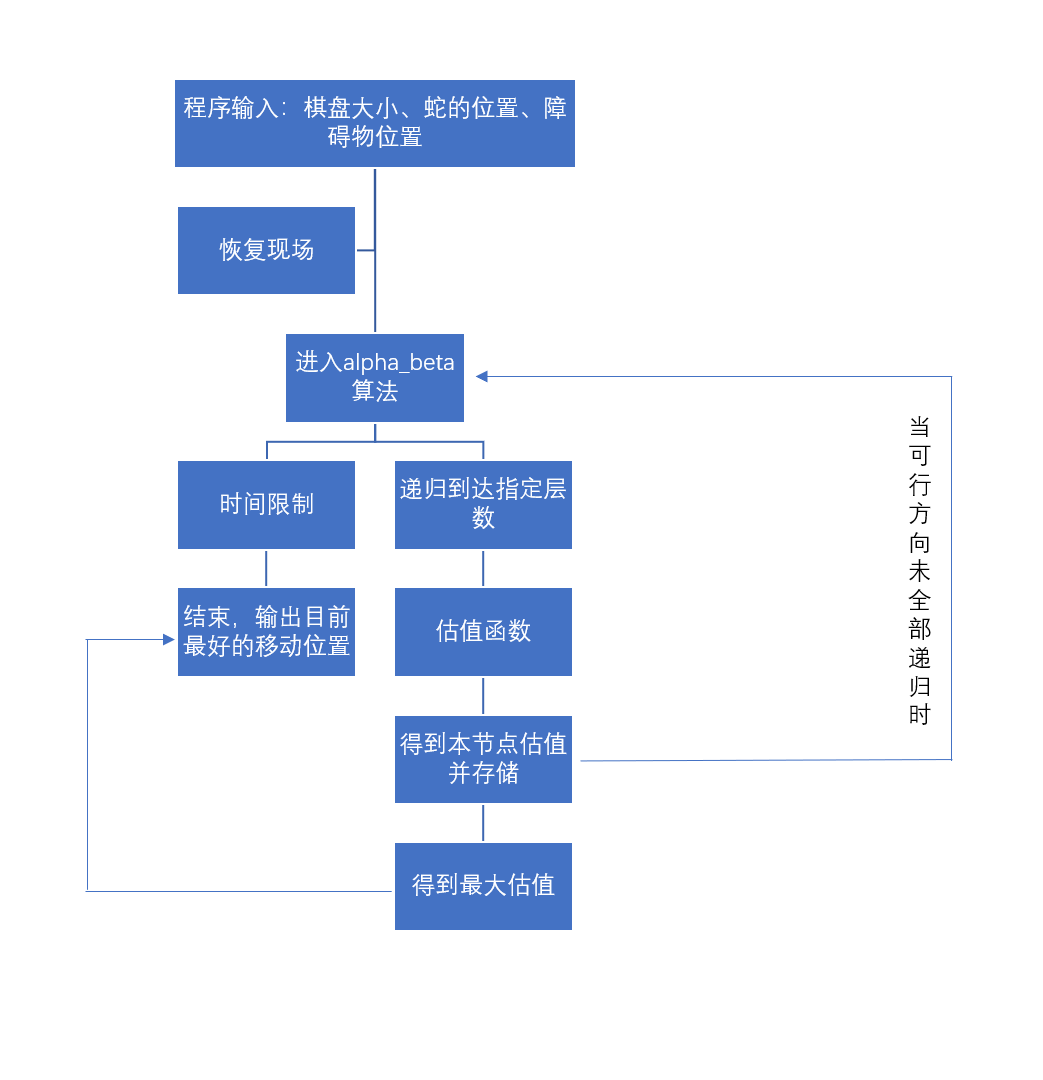
\includegraphics[width=1\textwidth]{1.png} %中括号中的参数是设置图片充满文档的大小,你也可以使用小数来缩小图片的尺寸。
    \caption{总图} %caption是用来给图片加上图题的
    \label{wolf} %这是添加标签,方便在文章中引用图片。
\end{figure}%figure环境



\begin{figure}[H] %figure环境,h默认参数是可以浮动,不是固定在当前位置。如果要不浮动,你就可以使用大写float宏包的H参数,固定图片在当前位置,禁止浮动。
    \centering %使图片居中显示
    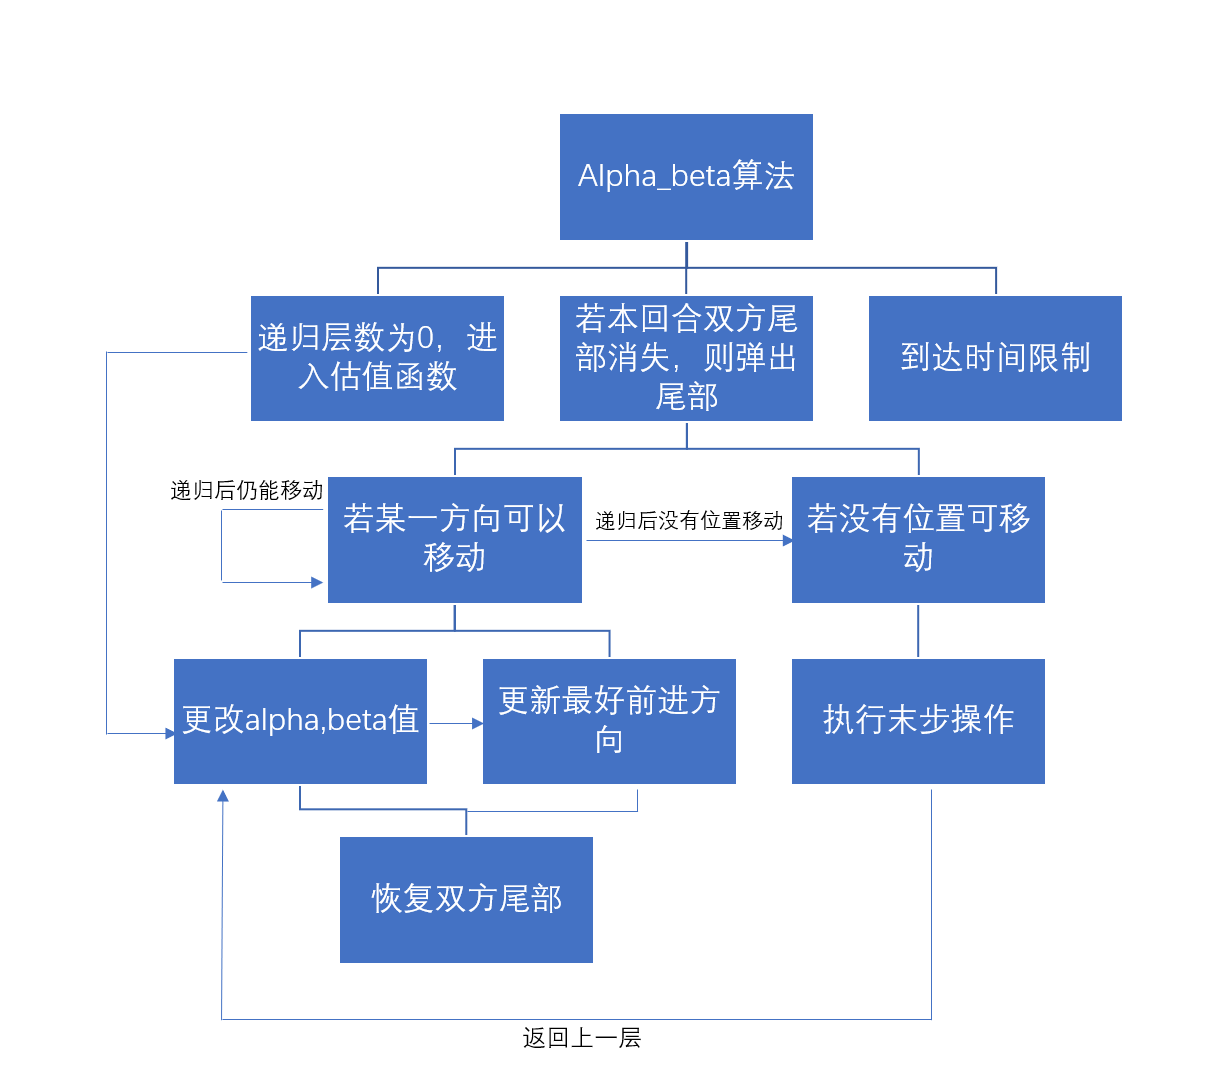
\includegraphics[width=0.9\textwidth]{2.png} %中括号中的参数是设置图片充满文档的大小,你也可以使用小数来缩小图片的尺寸。
    \caption{alpha-beta算法分图} %caption是用来给图片加上图题的
    \label{wolf} %这是添加标签,方便在文章中引用图片。
\end{figure}%figure环境

\begin{figure}[H] %figure环境,h默认参数是可以浮动,不是固定在当前位置。如果要不浮动,你就可以使用大写float宏包的H参数,固定图片在当前位置,禁止浮动。
    \centering %使图片居中显示
    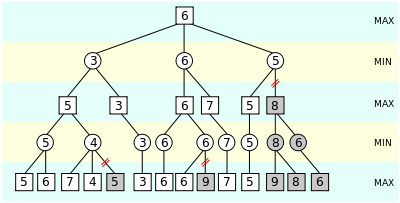
\includegraphics[width=0.6\textwidth]{3.png} %中括号中的参数是设置图片充满文档的大小,你也可以使用小数来缩小图片的尺寸。
    \caption{算法示意} %caption是用来给图片加上图题的
    \label{wolf} %这是添加标签,方便在文章中引用图片。
\end{figure}%figure环境


\section{算法运行时间复杂度分析}
Alpha-Beta 剪枝算法用于减小极大极小算法所搜索的节点数目,Alpha-Beta 剪枝算法的效率很大依赖于节点的排列,在理想的排序下,由
\begin{equation}
\label{eqn:eqn1}
O\left(\left(\left(b-1+\sqrt{b^{2}+14 b+1}\right) / 4\right)^{d}\right)\notag
\end{equation}


算法复杂度为$O\left(b^{d / 2}\right)$,可以使搜索节点的数量减小一半,从而使在相同时间下的搜索深度增加一倍。在随机排序下,算法复杂度平均为$O\left(b^{d *3/4}\right)$
最坏情况下,没有节点会被剪枝,整个树都会被检视,每个节点会检视$b^2$个子节点,最好情况下,每个结点都会检视$2b-1$个子节点。随意总的算法将会检验$O\left(b^{d / 2}\right)$ 个节点。

$d$:树的深度 

$b$:分支因子,是每个结点下的子结点数,即出度。

\chapter{程序代码说明}


\section{数据结构说明}
\vspace{1cm}
主要数据结构:
\vspace{0.4cm}

1. 采用了$c++$ $STL$ 类的list类型,对蛇体信息进行存储。
\vspace{0.4cm}

2. 用若干二维数组保存地图信息。
\vspace{0.4cm}

3. 用递归函数及回溯操作模拟博弈树,对博弈情况进行模拟和评估。

\section{函数说明}

\begin{lstlisting}[language=C++]
1. int evaluate(int total):
    int evaluate(int total)
{
	int dist1[25][25] = { 0 }, dist2[25][25] = { 0 }, temp_map[25][25];
	int st[25][25] = { 0 };

	for(int i=0;i<25;i++)
		for (int j = 0; j < 25; j++)
		{
			dist1[i][j] = 9999999;
			dist2[i][j] = 9999999;
			st[i][j] = 0;
		}
//对数组进行初始化st[数组]存放当前位置的点(不为零),表示蛇身体某点再经过几回合可以空出来。(存放回合数),dist1存放我方蛇局面评估信息,表示蛇头走到某点的回合数(dist2对方同理),dist1/2初始化为无穷大的目的:距离蛇头较近的点不一定先走,所以初始化每个点都无法达到。
	list<point>::iterator it0 = snake[0].end();
	list<point>::iterator it1 = snake[1].end();
	it0--;
	it1--;
	int k = 0;
	for (k = total - snake[0].size() + 1; k <= total; k++)
//k表示当前是第几个不增长的回合。
	{

		st[it0->x][it0->y] = disteps[k] - total;
//disteps相当于查表,disteps[i]内存放第i个不增长的回合
		st[it1->x][it1->y] = disteps[k] - total;
		if (it0 != snake[0].begin())
			it0--;
		if (it1 != snake[1].begin())
			it1--;

	}
//st[i][j]存放蛇身点(i,j)经过几回合后可以被使用(走)。
	general_map(temp_map);
//形成地图信息
	for (int id = 0; id <= 1; id++)
	{
		point head(snake[id].front());

		int visit[25][25] = { 0 };

		visit[head.x][head.y] = 1;
		if (id == 0)
			dist1[snake[id].front().x][snake[id].front().y] = 0;
		else
			dist2[snake[id].front().x][snake[id].front().y] = 0;

		deque<point> now_try;
//使用队列完成对于所有待评估点的遍历
		now_try.push_back(head);


		if (id == 0)
//对我方局面进行评估
		{
			while (!now_try.empty())
			{
				point new_p(*now_try.begin());
				now_try.pop_front();
				for (int d = 0; d < 4; d++)
				{
					point p1;
					p1.x = new_p.x + dx[d];
					p1.y = new_p.y + dy[d];

if (dist1[p1.x][p1.y] > dist1[new_p.x][new_p.y] + 1 && temp_map[p1.x][p1.y] != 1 && st[p1.x][p1.y] <= dist1[new_p.x][new_p.y] + 1)//
//st[p1.x][p1.y] <= dist1[new_p.x][new_p.y] + 1 表示当前蛇身的某点在经过dist[][]+1回合后空出来,可以使用。
					{
						now_try.push_back(p1);
						dist1[p1.x][p1.y] = dist1[new_p.x][new_p.y] + 1;

					}
				}

			}
		}

		if (id == 1)
		{
			while (!now_try.empty())
			{
				point new_p(*now_try.begin());
				now_try.pop_front();
				for (int d = 0; d < 4; d++)
				{
					point p1;
					p1.x = new_p.x + dx[d];
					p1.y = new_p.y + dy[d];

if (dist2[p1.x][p1.y] > dist2[new_p.x][new_p.y] + 1 && temp_map[p1.x][p1.y] != 1 && st[p1.x][p1.y] <= dist2[new_p.x][new_p.y] + 1)//
					{
						now_try.push_back(p1);
						dist2[p1.x][p1.y] = dist2[new_p.x][new_p.y] + 1;

					}
				}

			}
		}


	}





	int value1 = 0, value2 = 0;
	for (int i = 1; i <= n; i++)
		for (int j = 1; j <= m; j++)
		{
			if (dist1[i][j] < dist2[i][j])
//我方优势点
				value1 += dist_value[dist1[i][j]];//累计优势值
			else if (dist2[i][j] < dist1[i][j])
				value2 += dist_value[dist2[i][j]];

		}
	return value1 - value2;
////效益数组,越后走到的回合效益值越低



};
   
2. int alpha_beta(int depth, int id, int alpha, int beta, int total, bool firstpoint, int hash_value) 
int alpha_beta(int depth, int id, int alpha, int beta, int total, bool firstpoint, int hash_value) {
//firstpoint除了调用时赋值一,递归时赋值零,以标记第一层
	ret["response"]["total"] = total;
	

	if ((clock() - Time) >= timeout) //时间限制,在超时前结束
	
	{
		output(returnvalue);
		exit(0);

	}

	int now = -1000000000, bestmove = 0;
	int i, j;
	bool isdeletetail = 0;
	if (depth == 0) {//当递归剩余层数为0,进入估值函数
		return evaluate(total);
	}
	//----------------------------------------------
	int best = hash_move[hash_value & (HASH_SIZE - 1)];
     //从哈希表里取得最好移动方向

	/////

	point p0, p1;
	if (!whetherGrow(total)) {//尾部是否消失
		p0 = snake[0].back();//
		p1 = snake[1].back();//保存双方的尾部
	}

	int map[25][25];
	general_map(map);
	bool endflag = 1;//如果最后还是一,代表无路可走,调用末步函数
	if (!id)
	{

		if (whetherGrow(total) == 0)//若本回合双方尾巴消失
		{
			snake[0].pop_back();
			snake[1].pop_back();//消除尾部
		}
	}
	for (int i = best, j = 0; j < 4; i = (i + 1) & 3, j++)
	{
		point p = *(snake[id].begin());//读取目前前进的蛇最近移动的位置

		int snakex = p.x + dx[i];
		int snakey = p.y + dy[i];

		if (map[snakex][snakey] != 0) continue;//遇到障碍,不可前进到此处

		total = move1(id, i, total);//蛇移动
		int idnext = (id == 1 ? 0 : 1);
		endflag = 0;//目前还有某一方向可以走

		int score = -alpha_beta(depth - 1, idnext, -beta, -alpha, total, 0, hash_value * 20011 + i);//递归

		ret["response"]["score"] = score;


		if (id == 1) {//恢复模拟前的回合数
			total--;
		}
		snake[id].pop_front();//弹出模拟时放入的头部

		if (score > now) {
			bestmove = i;
			now = score;
			ret["response"]["now"] = now;
			if (alpha < score) {//剪枝
				alpha = score;
				if (firstpoint == 1) {
					returnvalue = i;
				}
			}
			if (score > beta) {//剪枝
				break;
			}
		}
	}
	if (endflag) {//末步函数
		now = noplace(id);//无路可走\成功处理
	}

	if (!id) {

		if (whetherGrow(total) == 0)//本回合消除了尾部
		{
			snake[0].push_back(p0);
			snake[1].push_back(p1);//恢复尾部

		}
	}


	hash_move[hash_value & (HASH_SIZE - 1)] = bestmove;//hash
	return now;
}







/*需要一个初始试探值,一般可以简单地选取初始搜索区间的中点,当然也可以根据具体情况选择对搜索更有利的值。
由于该算法必须采用散列表,散列表的性能对于整体算法的效率也是至关重要的。
另外,估值的取值范围大小,也会影响MTD(f)算法的搜索速度。
一般来说,估值越粗略(即取值范围较小),搜索速度会越快;这是由于试探的次数较少所致。
如果算法还涉及最佳棋步的求解,那么最佳棋步的取舍问题应引起注意。
虽然MTD(f)每进行一次零宽窗口试探,都会得到一个新的最佳棋步,但对于alpha节点(best_value < test时)。
我们所得到的“最佳棋步”只是满足估值上限的棋步,而非真正最佳的棋步。因此,我们应丢弃这种虚假的最佳棋步,而保留上一次搜索结果
*/
3. int mtd(int alpha, int beta, int depth, int test, int total)
{
	int best_value;
	do {
		// 进行零宽窗口试探
		best_value = alpha_beta(depth, 0, test - 1, test, total,1, 0);
		// 如果是alpha节点
		if (best_value < test) {
			// 更新估值上限,并将此做为新的试探值
			test = beta = best_value;
			// 否则是beta节点
		}
		else {
			// 更新估值下限
			alpha = best_value;
			// 新的试探值
			test = best_value + 1;
		}
	} while (alpha < beta);
	return best_value;
}

\end{lstlisting}
\section{程序限制}
若棋盘足够大回合足够多,例如出现某步可能需要蛇头部运行400步才能到达时,评估函数由于查表数组大小的限制,会出现失效。


\chapter{实验结果}



\section{测试数据}
将json格式字符串直接输入程序,进行单步执行。


\section{结果分析}
\begin{itemize}
    \item alpha-beta剪枝操作(主要时间开销)
    \item 缓存增强试探:大大提高了算法效率
    \item 局面评估函数:不仅针对当前场上可用的点进行评估,对于蛇体运动中即将空闲出来的点也有相应的评估。可实现预判蛇尾轨迹进行追尾部操作,使本方能获得更多的可能活动空间
\end{itemize}


\section{经典战局}
此算法程序在对战普通的未剪枝博弈树或普通剪枝博弈树或普通贪心或评估算法,具有较大优势,胜率较高。但若遇到完备的MCT算法的程序,则胜率大大下降。










{\let\clearpage\relax\chapter*{总结}}
%\chapter{总结}

这次课设让我们实践了数据结构课程的理论知识,并增强了我们对各种算法的理解与融会贯通。在网上查阅资料并相互讨论的过程中,我们接触到了新的方法如缓存增强试探法,散列表等,在这些方法的帮助下,提高效率,存储信息等问题得到了解决。但本算法仍然有改进空间,算法若采用全局的地图信息,则不必每次递归都形成一个新的地图状态,可微弱减少空间开销和时间开销。其次在团队协作编程时,务必要注意及时统一版本,避免出现重复劳动和代码版本混乱。在此次小组合作中,我们组内气氛融洽,小组成员都负责认真地完成了自己的任务,并充分与他人交流完成了代码对接,在交流沟通方面大家都获得了较大提升。













\chapter{参考文献}

\vspace{1.5cm}


\href{https://www.xqbase.com/computer/search_alphabeta.htm
}{https://www.xqbase.com/computer/search_alphabeta.htm
}
\vspace{0.7cm}

\href{http://www.soongsky.com/othello/computer/mtdf.php
}{http://www.soongsky.com/othello/computer/mtdf.php
}
\vspace{0.7cm}

\href{http://www.soongsky.com/othello/computer/alpha_beta.php
}{http://www.soongsky.com/othello/computer/alpha_beta.php
}
\vspace{0.7cm}

\href{http://www.soongsky.com/othello/computer/hashtable.php
}{http://www.soongsky.com/othello/computer/hashtable.php
}

\bibliographystyle{plain}
\bibliography{ref}
\bibliography{Reference.bib}
  


\end{document}